\def\theTopic{t Procedures for a Single Mean }
\def\dayNum{23 }


\begin{center}
 {\large \textbf{t-Distributions - Inference for One Mean}}
\end{center}


In a previous semester, we asked STAT216 students to estimate how much they were
spending on textbooks during that semester.  We had sample size 319
with mean $\xb = 329.44$ and spread $s = 202.93$ (both in
dollars). Here is a histogram of 
the individual data and another of 5000 resampled means.

% bookCost <- read.csv("../../data/Cost of Books.csv")
%  sd(bookCost$cost)##[1] 202.9328 
% summary(bookCost$cost)
% #    Min.  1st Qu.   Median     Mean  3rd Qu.     Max. 
% #   0.001  200.000  300.000  329.400  450.000 1000.000 
%  dim(bookCost)  # [1] 319   3 

%  stackPlot <- function(x, breaks, slant = FALSE){
%     ## function to plot stacks of dots
%     cutGroups <- cut(x, breaks)
%     x <- sort(x)
%     if (!slant){
%       levels(cutGroups) <- round(tapply(x, cutGroups, mean))
%       x <- as.numeric(as.character(cutGroups ))
%     }
%     y <- unlist(tapply(x, cutGroups, function(z) 1:length(z)))
%     plot(x, y, main = paste("Distribution of Resampled Means"), xlab = "", ylab = "Frequency")
%      }
% #stackPlot(bootMeans, 20)
% par(mfrow=c(1,2), mar = c(4,1,1,1))
%  hist(bookCost$cost,breaks = 15,xlab="Textbook Cost for 1 Semester at MSU", main ="Individual Book Costs", yaxt="n", ylab = '')
% bootMeans <- apply(matrix(sample(bookCost$cost, 5000*319,
% replace=TRUE),5000, 319),1,mean)
% hist(bootMeans, main = "Bootstrap Means With t(318)", xlab="Resampled Means", yaxt="n", ylab = '', probability=TRUE)
%  curve(dt((x-329.4)/ 11.2, 318)/11.2,add=TRUE)
% dev.copy(png,file="plots/bookCostDistns.png", height = 300, width =
% 650);dev.off()
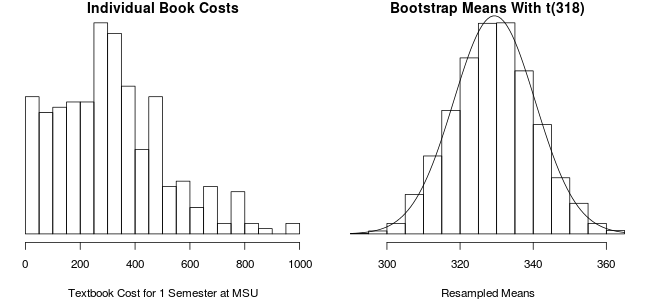
\includegraphics[width=\linewidth]{plots/bookCostDistns.png}
The second plot is overlaid with a $t_{318}$ density curve.  Note how
it gives a very similar distribution to the bootstrap resampled means,
even though the original data is not symmetric.

We needed many bootstrap samples to get what the web app called
``standard deviation'' of the resamples.  Now we will use a
formula for the standard error (SE) of the sample mean, $\xb$ based on
sample size and the standard deviation of the raw data.  
$$SE(\xb) = \frac{s}{\sqrt{n}}$$
In the left-hand plot above, the spread of the individual points is $s
= 202.93$. The resampled means have spread of 11.20 which is quite
close to $SE(\xb) = 202.93/\sqrt{319} = 11.36$.  
\begin{itemize}
\item {\bf Standard Deviation} has several meanings:
  \begin{itemize}
    \item the spread of some  distribution, especially: the spread of
      individual  measurements.
    \item Population standard deviation with  Greek letter: $\sigma$,
    \item Sample standard deviation, $s$ from the formula: $s =
      \sqrt{\frac{1}{n-1}\sum(x_i - \xb)^2}$
    \item  Standard deviation of a statistic, for instance  $SD(\xb)
      =\sigma/\sqrt{n}$, is the true spread of the statistic.
  \end{itemize}

\item {\bf Standard error} is the estimated standard deviation of a
  statistic. Below is a table of the  standard deviations and standard
  errors we  are using.  Note how the SE just plugs an estimated value
  in to the SD formula.\\
  \begin{center}
  \begin{tabular}{|c|c|c|}\hline
    Statistic: & Standard Deviation & Standard Error\\ \hline
    $\phat$ & $\sqrt{\frac{p(1-p)}{n}}$ & $\sqrt{\frac{\phat(1-\phat)}{n}}$\\
    \hline
    $\phat_1 - \phat_2$&  $\sqrt{\frac{p_1(1-p_1)}{n_1}
      +\frac{p_2(1-p_2)}{n_2} }$ & $\sqrt{\frac{\phat_1(1-\phat_1)}{n_1}
      +\frac{\phat_2(1-\phat_2)}{n_2} }$\\ \hline
     $\xb$ & $\frac{\sigma}{\sqrt{n}}$ & $\frac{s}{\sqrt{n}}$ \\\hline
     $\xb_1 - \xb_2$ & $\sqrt{\frac{\sigma_1^2}{n_1} +\frac{\sigma_2^2}{n_2}} $
      & $\sqrt{\frac{s_1^2}{n_1} +\frac{s_2^2}{n_2}} $  \\ \hline
  \end{tabular}\vspace{.1in}    
  \end{center}
\end{itemize}

  Each of these $SD$'s and $SE$'s has sample size (square
  rooted) in the denominator.  As sample size gets big, $SD$ and $SE$ get
  smaller. More information leads to less variation.

  Add to this the fact that sample mean is an {\bf unbiased} estimator
  of the true population mean, and sample proportion is an {\bf
  unbiased} estimator of the true population proportion, and we see
  the power of using statistics to estimate parameters: larger sample
  sizes provide more information, less variation, and we can close in
  on the true parameter values. Here are two big ideas in statistics:

  \begin{center}
    {\large \bf  Law of Large Numbers}\vspace{.2cm}
\\
 \begin{fmpage}{.9\linewidth}
  In the long run, the sample mean $\xb$ will get closer and closer to the
   population mean, $\mu$, and the sample proportion $\phat$ will get
   closer and closer to the true proportion of successes, $p$.  You can define
   ``close'' as you wish -- smaller values just mean we'll need larger
   sample sizes.
 \end{fmpage}
  \end{center}
 
  The second important idea addresses the {\bf shape} of the sampling
  distribution, and was more of a surprise when it was discovered
  about 200 years ago (and proven, in general only 100 years ago). 

  \begin{center}
    {\large \bf  Central Limit Theorem} \vspace{.2cm}
\\
\begin{fmpage}{.9\linewidth}
  As the sample size gets big, the shape
  of the sampling distribution of sample mean, $\xb$ gets closer and
  closer to a normal distribution.
\end{fmpage}
  \end{center}

This explains why the normal distribution is so useful.  Even if we
start with skewed data, like in the case of book costs, when we
average together 100 or more random values, the distribution of the
sample mean, $\xb$,  will approach a normal distribution.  It also
applies to proportions because if we record success as 1 and failure as
0, then $\phat$ is just the sample mean of the zeroes and ones.


%% Galton's Board here?


\begin{center}
  {\large\bf Assumptions for t-Procedures}
\end{center}

  Just as with proportions, all means methods require 
  \begin{itemize}
     \item The size of each sample must be less than a tenth the size
       of its population.
     \item Each sample must be representative of its population. 
     \item Independent samples and independent subjects within each
       sample.
  \end{itemize}
   In addition, we do need to examine the sample size {\bf and} shape
   of the sample data to determine if we can use $t$ procedures.
   \begin{itemize}
   \item For small sample sizes, we need distributions to be close to
     normally distributed: symmetric with no outliers.
   \item If sample size is 30 or more, we can use $t$ procedures
     unless the data are heavily skewed.
   \item If sample size is over 100, the Central Limit Theorem lets us
     use $t$ distributions even for heavily skewed data.
   \end{itemize}

   \begin{center}
     {\large\bf True or False:}
   \end{center}
   \begin{enumerate}
   \item \underline{\hspace{.5in}} The Law of Large Numbers says that the
     distribution of $\xb$  gets close to normal as $n$ gets big. 
   \item \underline{\hspace{.5in}} As degrees of freedom get big,
     $t$-distributions get 
     closer and closer to the standard normal distribution.
   \item \underline{\hspace{.5in}} The Central Limit Theorem gives us the shape of
     the distribution of $\xb$ for large $n$.
   \item \underline{\hspace{.5in}}  With larger sample size, we have better
     information about population parameters.
   \item \underline{\hspace{.5in}} Statistics from larger samples are less biased
     than those from smaller samples.
   \end{enumerate}

\begin{center}
  {\large\bf Confidence Interval for $\mu$}
\end{center}

With text book costs, we had:
$$ n = 319, \mbox{\hspace{1in}} \xb = 329.44, \mbox{ and\hspace{1in}}  s = 202.93 $$

With one sample, we use $n-1$ as the ``degrees of freedom'' for the t
distribution.  
\begin{enumerate}
  \setcounter{enumi}{5}
  \item Use the web app \url{http://shiny.math.montana.edu/prob} 
    to find the $t^*_{318}$ multipliers to use in the formula for
     confidence interval:
     $$  \mbox{estimate} \pm t^*_{df} SE(\mbox{estimate}) $$
\begin{students}
   \begin{tabular}{l|rrrrr}
    Confidence level: &  \hspace{1cm}80\% &  \hspace{1cm}90\% &  \hspace{1cm}95\% & \hspace{1cm} 98\% & \hspace{1cm} 99\% \\ \hline
    $t_{318}^*$ cutoff  &  &  & 1.967 &  & 
  \end{tabular}\vspace{.2cm}
\end{students}
\begin{key}
   \begin{tabular}{l|rrrrr}
    Confidence level: &  \hspace{1cm}80\% &  \hspace{1cm}90\% &  \hspace{1cm}95\% & \hspace{1cm} 98\% & \hspace{1cm} 99\% \\ \hline
    $t_{318}^*$ cutoff  &1.284  &1.65  & 1.967 &2.338& 2.591
  \end{tabular}\vspace{.2cm}
\end{key}
   (Do change from \fbox{Normal} to \fbox{t} distribution, and set
   degrees of freedom to 318.)
 \item 
   How different are these from the values you found for the z
   distribution last week?
\begin{students}
  \vspace{1cm}
\end{students}
\begin{key}
\\ {\it Just a touch wider}
\end{key}
\item Find the margin of error and build a 90\% confidence interval
  for the true book cost.   
\begin{students}
  \vspace{1cm}
\end{students}
\begin{key}
\\ ME = $ 1.65 \times 202.93\sqrt{319} =18.747$ the 90\% CI is $
329.44 \pm 18.747 = (310.69, 348.19)$
\end{key}
\item Interpret the interval. 
\begin{students}
  \vspace{1cm}
\end{students}
\begin{key}
\\ {\it We are 90\% confident that the true mean amount spent on
  textbooks by some group of students is between \$310.69 and \$348.19.}
\end{key}
\item To what group of students does this inference apply? 
\begin{students}
  \vspace{1cm}
\end{students}
\begin{key}
\\ {\it Trick question: This was not a random sample of MSU
  students. It really just applies to the students in the sample.}
\end{key}

\end{enumerate}


\begin{center}
  {\large\bf Hypothesis Test}
\end{center}
We do not have a hypothesized value to use for true mean textbook
cost, so let's look at a different situation to do a hypothesis test
on one mean.  An article in the {\it Journal of American Medical
  Association} in 1992 provided data to challenge the long held belief
that ``normal'' human body temperature is $98.6^o$F.\footnote{
Mackowiak, P. A., Wasserman, S. S., \& Levine, M. M. (1992). A
critical appraisal of 98.6 F, the upper limit of the normal body
temperature, and other legacies of Carl Reinhold August
Wunderlich. {\it JAMA}, 268(12), 1578-1580.}  Research before this study was
published led the researchers to believe that ``normal'' for most
people is lower than $98.6^o$.


\begin{enumerate}
\setcounter{enumi}{5}
\item  What are the null and alternative hypotheses?  
\begin{students}
\\$H_0$:  \vspace{1cm}\\
$H_a$:  \vspace{1cm}
\end{students}
\begin{key}
\\ $H_0:\ \ \mu = 98.6$\\
$H_a:\ \ \mu<98.6$
\end{key}

Check these with another group at your table, because being off on
direction will mess us up later.

\item  
Go to the Rossman-Chance site, pick \underline{Descriptive
  Statistics}, clear their data, and enter these values:
\begin{verbatim}
temp
97.3 97.3 97.7 97.8 98.4 99.8 96.7 98.1 98.7 97.5
97.9 98.1 97.8 98.5 98.8 98.7 99.4 97.8 98.6 98.7
\end{verbatim}
 Find the mean and standard deviation ($s$). Use 3 decimal
  place accuracy throughout.
\begin{students}
  \vspace{1cm}
\end{students}
\begin{key}
\\ $\xb = 98.18$,  $s = 0.747$
\end{key}

\item Compute $SE(\xb)$.
\begin{students}
  \vspace{1cm}
\end{students}
\begin{key}
\\ {\it $0.747/\sqrt{20} = 0.167$}
\end{key}

\item How many standard errors is $\xb$ from $\mu_0$?  Compute the
  test statistic. 
\begin{students}
  \vspace{1cm}
\end{students}
\begin{key}
\\ {\it $ \frac{98.180 - 98.6}{0.167} = -2.514$}
\end{key}


\item Which $t$ distribution should we use?
\begin{students}
  \vspace{1cm}
\end{students}
\begin{key}
\\ {\it $t$ with 19 df}
\end{key}



\item Go back to \url{http://shiny.math.montana.edu/prob} 
  and put the t-statistic into the top
  box. Change the distribution to \fbox{t} and set the degrees of
  freedom you found just above. Check the direction of your
  alternative hypothesis and give the p-value for the test.
\begin{students}
  \vspace{1cm}
\end{students}
\begin{key}
\\ {\it 0.011}
\end{key}
\item  How strong is the evidence against $H_0$?  State your
  conclusion at the $\alpha = 0.04$ significance level.
\begin{students}
  \vspace{1cm}
\end{students}
\begin{key}
\\ {\it Very strong. We reject $H_0$ and conclude that true mean
  ``normal'' body temperature is less than $98.6^o$ F}
\end{key}

\item Based on your p-value, will a 96\% confidence interval for true
  mean body temperature contain 98.6?
\begin{students}
  \vspace{1cm}
\end{students}
\begin{key}
\\ {\it No. It is not a plausible value based on this sample.}
\end{key}

\item Build the 96\% CI.  Be sure to show which $t^*$ you use.
\begin{students}
  \vspace{1cm}
\end{students}
\begin{key}
 {\it $t^*_{19} = 2.2047$, 96\% CI $= 98.18 \pm 2.2047 \times 0.167 =
   (97.81, 98.55)$} 
\end{key}

\item Write up a report on  your hypothesis test of ``Normal'' body
  temperature.  You 
  may assume that these temperatures are from a random sample of US
  men and women aged 20 to 40 years old. (With one only group we do not make
  comparisons in the report.)

\end{enumerate}



\begin{center}
  {\large\bf Take Home Message}
\end{center}
 
\begin{itemize}
\item Larger sample sizes are generally better than smaller ones --
   as long as they are representative.  If we are using a biased
   sampling method, no amount of increase in sample size will fix the
   bias problem.
 \item As sample size, $n$ gets big:
   \begin{itemize}
   \item statistics get closer to their respective parameters.
   \item distributions of means get closer to normal in shape.
   \item t-distributions get closer to Z (N(0,1)) because degrees of
     freedom are related to sample size.
   \end{itemize}
 \item Generic confidence interval:
  $$ \mbox{estimate} \pm \mbox{multiplier} SE(\mbox{estimate})$$
    for a single mean:
  $$ \xb \pm t^*_{n-1} SE(\xb)$$
  \item Test statistic:
   $$ t = \frac{\xb - \mu_0}{SE(\xb)};\ \ SE(\xb) =
   \frac{s}{\sqrt{n}}$$
    Compare to a $t_{n-1}$ distribution to get p-values.

 \item What questions do you have?  Write them here.

\end{itemize}




%% 4 pages. Too short? Add Galton's bd? est assumptions.